\documentclass[conference]{IEEEtran}
\IEEEoverridecommandlockouts
% The preceding line is only needed to identify funding in the first footnote. If that is unneeded, please comment it out.
% \usepackage{cite}
\usepackage{amsmath,amssymb,amsfonts}
\usepackage{algorithmic}
\usepackage{graphicx}
\usepackage{textcomp}
\usepackage{xcolor}
\def\BibTeX{{\rm B\kern-.05em{\sc i\kern-.025em b}\kern-.08em
    T\kern-.1667em\lower.7ex\hbox{E}\kern-.125emX}}
\usepackage[acronym]{glossaries}    % acronyms/ abbreviations

\usepackage[style=ieee]{biblatex} %Imports biblatex package
\addbibresource{main.bib} %Import the bibliography file


% acronyms
\makeglossaries
\newacronym{nft}{NFT}{Non-fungible Token}
\newacronym{ml}{ML}{Machine Learning}
\newacronym{dl}{DL}{Deep learning}
\newacronym{ai}{AI}{Artificial Intelligence}
\newacronym{nlp}{NLP}{Natural Language Processing}
\newacronym{erc}{ERC}{Ethereum Request for Comments}
% \newacronym{gui}{GUI}{Graphical User Interface}
% \newacronym{p@k}{P@K}{Precision at K}
% \newacronym{mse}{MSE}{Mean Squared Error}
% \newacronym{rmse}{RMSE}{Root Mean Square Error}
% \newacronym{mae}{MAE}{Mean Absolute Error}
% \newacronym{mlp}{MLP}{Multilayer Perceptron}
\newacronym{lstm}{LSTM}{Long short-term memory}
\newacronym{api}{API}{Application Programming Interface}
% \newacronym{rnn}{RNN}{Recurrent Neural Network}
% \newacronym{ide}{IDE}{Integrated Development Environment}
\newacronym{recsys}{RecSys}{Recommendation System}
    
\begin{document}



\title{An Adaptive Approach for Generalized Text Summarization using Optimized Transformers\\
% {\footnotesize \textsuperscript{*}Note: Sub-titles are not captured in Xplore and
% should not be used}
% \thanks{Identify applicable funding agency here. If none, delete this.}
}

\author{\IEEEauthorblockN{Nazhim Kalam}
\IEEEauthorblockA{\textit{Computer Science and Engineering} \\
\textit{University of Westminster}\\
London, UK \\
nazhimkalam@gmail.com}
\and
\IEEEauthorblockN{Torin Wirasingha}
\IEEEauthorblockA{\textit{Department of Computing} \\
\textit{Informatics Institute of Technology}\\
Colombo, Sri Lanka \\
torin.w@iit.ac.lk}
% \and
% \IEEEauthorblockN{3\textsuperscript{rd} Given Name Surname}
% \IEEEauthorblockA{\textit{dept. name of organization (of Aff.)} \\
% \textit{name of organization (of Aff.)}\\
% City, Country \\
% email address or ORCID}
% \and
% \IEEEauthorblockN{4\textsuperscript{th} Given Name Surname}
% \IEEEauthorblockA{\textit{dept. name of organization (of Aff.)} \\
% \textit{name of organization (of Aff.)}\\
% City, Country \\
% email address or ORCID}
% \and
% \IEEEauthorblockN{5\textsuperscript{th} Given Name Surname}
% \IEEEauthorblockA{\textit{dept. name of organization (of Aff.)} \\
% \textit{name of organization (of Aff.)}\\
% City, Country \\
% email address or ORCID}
% \and
% \IEEEauthorblockN{6\textsuperscript{th} Given Name Surname}
% \IEEEauthorblockA{\textit{dept. name of organization (of Aff.)} \\
% \textit{name of organization (of Aff.)}\\
% City, Country \\
% email address or ORCID}
}

\maketitle

\begin{abstract}
This research explores the ways in which to get an optimal solution using Transformer for abstractive text summarization and yet making a generalized solution that can be adapted with respect to any domain (be it hotels, movies, restaurants) and increase its performance as the system gets used over time.
% human-computer interaction.
\end{abstract}

\begin{IEEEkeywords}
Natural Language Processing, Machine Learning, Deep Learning, Recall-Oriented Understudy for Gisting Evaluation, Inductive logic programming
\end{IEEEkeywords}

% SECTION #1
\section{Introduction}
Today, there is a lot of textual material available, including news stories and reviews. Text summarizing helps us quickly find the key elements of the full piece by minimizing the quantity of text. \cite{etemad_abidi_chhabra_2021}. Transformers in NLP is a novel architecture that aims to solve sequence-to-sequence tasks while handling long-range dependencies with ease. It has surpassed competing neural models like CNN (Convolutional Neural Nets) and RNN (Recurrent Neural Nets) in terms of performance to appear as the dominant architecture for natural language processing \cite{wolf__2020}.

\subsection{User Reviews}
A user/customer review is typically referred to be written feedback from a customer who has used a product or service. Consumers frequently use user ratings and reviews to drive their purchasing decisions. Because the review data is unstructured, it becomes more challenging for consumers to compare and understand lengthier reviews \cite{mcauley_leskovec_2013}

User and customer reviews are extremely important to major corporations like tourism and hospitality, as they constitute the primary engine for the country's economic growth and development. where tourists from over the world may blog about their experiences and share their reviews online in numerous formats \cite{mukherjee_peruri_vishnu_goyal_bhattacharya_ganguly_2020}. 

\subsection{Corporate Advantage}
It is also known that it costs at least five times as much time and money to acquire a new customer as it does to keep an existing one, so it is important to learn how to foster customer loyalty to the brand, business, or service that is being offered. Customer satisfaction is essential to the survival of corporate industries. Understanding client expectations through their feedback or reviews helps business industries grow and fix faults \cite{pizam_ellis_1999}.

On the other hand, companies like Netflix or Amazon Prime can use movie summaries to help users understand their watching pattern or their interest. Likewise, movie-related industries need to allow customers to quickly scan the summary and quickly decide whether they should be watching it or not \cite{khan_gul_zareei_biswal_zeb_naeem_saeed_salim_2020}.

\subsection{Text Summarization}
With the massive accumulation of information/data on the internet nowadays, it is extremely difficult to extract relevant information from numerous textual documents. The goal of text summarizing is to provide a condensed yet meaningful version of lengthy textual content \cite{shi_keneshloo_ramakrishnan_reddy_2020}. 

We all know that text summarization has several uses in a variety of internet-based fields, including search engines that are used for querying and e-commerce sites that utilize sentiment analysis to determine client satisfaction with items \cite{etemad_abidi_chhabra_2021}.

However, in the movie industry, consumers may utilize text summarization to simplify customer reviews of movies, which are often lengthy and time-consuming to read. This enables users to make better decisions when they decide whether to watch a certain movie \cite{khan_gul_zareei_biswal_zeb_naeem_saeed_salim_2020}.

\subsection{Abstractive and Extractive Techniques}
Generally, text summarization is classified into two which are; abstractive text summarization and extractive text summarization, however, the approach for creating a hybrid model for text summarization is possible \cite{alsaqer_sasi_2017}. The abstractive text summarization technique aims to produce sentences on its own and then uses them to provide a coherent summary. Therefore, the summary's content will vary from the original context yet still convey the same idea \cite{etemad_abidi_chhabra_2021}. Additionally, it is well-recognized that a strong abstractive summary encompasses the input's key details and is linguistically fluent \cite{zhang_xu_wang_2019}.

The extractive text summarizing method focuses on picking out key phrases or groups of phrases from the original input content and combining them to produce a concise yet insightful text summary. It is determined which sentences should be included as parts of the summary based on the statistical and linguistic characteristics of the sentences \cite{gupta_lehal_2010}. A hybrid system is one that combines various strategies to produce a single system. However, hybrid text summarizing systems do exist, for instance, using a combination of extractive and abstractive summarization can be utilized to generate a hybrid system that uses encoder-decoders \cite{kirmani_manzoor}

\subsection{NLP with Deep Learning}
NLP is a method for computers to intelligently and effectively analyze, comprehend, and derive meaning from human language, as opposed to other approaches that only focus on the interactions between human language and computers. Deep learning techniques are increasingly being used in the field of AI compared to traditional machine learning approaches due to their success rates in handling difficult high-computing learning tasks \cite{lopez_kalita_2017}.

In today's NLP, machine learning is prominent, but for the most part, it only involves numerically optimizing the weights of characteristics and representations that have been created by humans. Deep learning aims to investigate how computers can utilize data to create features and representations suitable for challenging interpretation tasks \cite{socher_bengio_manning}.

\subsection{Transformers}
The open-source library Transformers contain modern transformer architectures that have been thoroughly developed and are integrated by a common API. Pretraining has enabled the efficient use of this capacity for a wide range of activities, and these designs have permitted the construction of higher-capacity models. Transformers are designed to be easy for practitioners, expandable for researchers, and quick and reliable in industrial deployments \cite{wolf__2020}.

It has been demonstrated that the modern generation of pre-trained language models based on transformers is rather competent at identifying syntactic signals like noun modifiers, possessive pronouns, prepositions, or co-referents, as well as semantic cues like entities and relations \cite{brasoveanu_andonie_2020}. Hugging Face Hub offers a variety of transformer designs, including BERT, GPT2, T5, PEGASUS, and many others. The figure below represents the daily average for unique downloads of the pre-trained transformer model architectures between Oct 2019 to May 2020 \cite{wolf__2020}. 

\cite{etemad_abidi_chhabra_2021} the research compares various other researchers' approaches taken in order to perform abstractive text summarization, these techniques include the use of transformers and other neural networks approach such as CNN and LSTM RNN networks. The research comparison table below only includes the approaches of transformers used, taken in abstractive text summarization.

\subsection{Hyperparameter Tuning}
Finding the ideal collection of parameter values to train an algorithm using in order to build a model relevant to the dataset is known as hyperparameter tuning \cite{liu_wang_2021}. The calculation of the performance improvement that may be obtained by changing the value of each of the considered hyperparameters from the original value to the value indicated in the target configuration set by the tuning strategy is where hyperparameters make the biggest contribution to improving algorithm performance \cite{joy_selvan_2022}. 

There are several hyperparameters that play a significant role in performance enhancement; however, not all the parameters do so; just a select handful do, for example, learning rate, weight decay, number of epochs, batch size, and warm-up ratio. As a result, giving critical hyperparameters a higher priority is crucial \cite{engdahl_2008}.

Automated framework tools, such as Optuna, an open-source framework for hyperparameter optimization built on the Python programming language, do hyperparameter tweaking. The application of numerous hyperparameter optimization techniques, including Grid Search, Random Search, TPE, and CMA-ES algorithms, was made easier by this framework \cite{joy_selvan_2022}.

\subsection{Generalization}
Generalization now plays a significant part in resolving issues in numerous fields that are linked to the same issue. The capacity of a model to generalize to new, previously unobserved data that comes from the same distribution as the model's original data is known as a generalization \cite{etemad_abidi_chhabra_2021}. 

Generalization is a useful strategy for starting with the foundation and improving or specializing in one's field as more unseen domain data becomes available. Therefore, the generalized solution will be able to adapt to even unseen domain data, making this solution solve a common problem in multiple domains \cite{Zhou_2021}.

\subsection{Data Expansion}
The quality of a machine learning or deep learning model depends on a number of factors, one of which is the amount and quality of data fed during model training. There are several approaches to increase or expand your available data, one of which is data augmentation (making use of existing data points to create new data points). Making use of new data from the user end by saving as the model is used is another way of exposing new data for model retraining \cite{barna_heickal_2022}. When generalized models are required to adapt to become domain-specific, model retraining will be considered with new data used by the specialized domain as the application is used.

% SECTION #2
\section{Motivation to enhance abstractive text summarization performance}

The identified problem can also be applied to several other domains which require improving the quality of abstractive text summarization using the advanced approaches of deep learning, not only specific movie reviews, this is why a generalized solution was thought of initially \cite{kouris_alexandridis_stafylopatis_2019}. 

As mentioned in the work of \cite{etemad_abidi_chhabra_2021}, syntactic and semantic issues with text summarization were the main issues that researchers were concerned with solving. and with respect to their research by exploring multiple deep learning techniques, they concluded that Transformer based models (T5 model) outperformed in all NLP tasks, this encourages the author to go deeper into the field of transformers optimization in order to enhance the quality of text summarization and address the constraints associated with the summarizing of movie reviews.

In the domain of movie review summarization, currently, there is no research done using the latest deep learning approaches (such as Transformers) to solve this problem, standard machine \& deep learning algorithms such as Naïve Bayes, and RNN has been used, and the usage of advanced deep learning approaches can be utilized in order to enhance the quality/accuracy of the text summarization.

Deep learning models take longer to train, but they provide greater accuracy since they can simultaneously automate feature extraction and classification, whereas machine learning algorithms require feature selection at first. Therefore, applying deep learning techniques will help to improve the quality of text summarization and help the user in making better decisions \cite{etemad_abidi_chhabra_2021}.

% SECTION #3
\section{Existing Work}

\subsection{Text Summarization Systems}

There were multiple studies done previously in the area of text summarization, regarding both abstractive and extractive text summarization. \cite{khan_gul_zareei_biswal_zeb_naeem_saeed_salim_2020} research is related to the domain of movie reviews summarization which is the same as this project domain, where the author has developed an automatic approach to summarize lengthy movie reviews along with a feature where the users are allowed to quickly recognize the positive and negative aspects of the movie with respect to the review process with. The text summarization approach taken by the author is an extractive approach, where sentence score ranking plays a major role in creating the summary.

The study of \cite{boorugu_ramesh_2020} is towards the domain of e-commerce but yet related to text summarization for customer reviews on the products they sell, so the purpose is that allow other customers to make better purchasing decisions on products, therefore the hassle of going through all the reviews to making a purchasing decision can be reduced to save time, the abstractive approach is considered to create the summary, which is a better choice of approach.

The research of \cite{mukherjee_peruri_vishnu_goyal_bhattacharya_ganguly_2020} is another extractive approach for text summarization, where the author develops a solution for generating personalized aspect-based opinion summaries using a  dataset that consists of a large collection of online tourist reviews. In addition, the author has gone a step further to personalize the summary's qualities by using the user's interest. However, using abstractive summarization would be a more effective strategy but also challenging when user interest customization is considered because the sentences have been created using their own words rather than with any sentence ranking technique.

\cite{gupta_lehal_2010} research is a comprehensive comparison study with benchmarking results of various pre-trained transformer architectures such as BART, BERT, T5, PEGASUS, etc... for abstractive text summarization which is an abstractive approach. This study includes the various types of datasets used to explore each model, with the evaluations as benchmarking results. The author has also concluded the best-performing transformer architecture as T5 by comparing the evaluation results of the study. 

The study conducted by \cite{etemad_abidi_chhabra_2021} is also an abstractive approach to text summarization with the addition of proper grammar and no repeated words used a deep learning approach with RNN and likewise \cite{etemad_abidi_chhabra_2021} research also relates to an experimenting study with various deep learning approaches for abstractive text summarization along with the evaluation benchmarking with a  goal in search for the best deep learning approach for the problem.

\subsection{Algorithmic approaches for Text Summarization}
The study of \cite{khan_gul_zareei_biswal_zeb_naeem_saeed_salim_2020} starts by first focusing on feature extraction, then transforming reviews into vector spaces, and applying the Naive Bayes machine learning method for review classification utilizing an undirected weighted graph-based ranking algorithm to rank score for each review phrase in graph and then, in order to construct the extractive summary, the highest scoring sentences are selected. However, the author has limited the use of sophisticated deep learning algorithms to improve performance by solely using standard machine learning approaches to tackle the problem.

\cite{boorugu_ramesh_2020} research made use of the seq2seq model for text summarization along with the attention mechanism for improved accuracy and the concept net number batch word embedding model, which is superior to the glove. Utilizing a 1D convolutional layer, a max pooling layer, an LSTM layer, and finally a fully connected layer at the very end. However, the author's use of generic deep learning algorithms to handle this problem introduces a new constraint that prevents performance from being improved using the most recent deep learning strategy for NLP-related problems, transformers.

The study of \cite{etemad_abidi_chhabra_2021} focuses on the author's study utilizing the encoder-decoder model with the attention layer to produce text summaries with good syntax and no repeated words. The creation of an encoder-decoder model with gated recurrent units and training it to provide an abstract summary of a piece of writing. Although the author employed deep learning, its application in production required real-time training so that it could be updated with the most recent content over time.

\subsection{Usage of Transformers}
\cite{gupta_lehal_2010} The research employed pre-trained models such as Pipeline BART, BART modified, T5, and PEGASUS to deal with text summarization as a part of the comparison study done. The ROUGE Scores were used as the evaluation measures. During the experiments, the author employed transformer designs; however, the hyperparameters used were defaulted and might be tuned for better performance. The constraints consist of concentrating on developing more reliable models that can further expand the method to produce summaries of varying lengths and applicable for multi-document summarization.

\cite{etemad_abidi_chhabra_2021} The author explores deep learning methods in the broad text summarization domain to determine which method—among a collection that includes RNN, CNN, and Transformers—performs best. The author also considers metrics for model evaluations including BLEU and ROUGE, despite using sophisticated deep learning algorithms, the author was unable to undertake hyperparameter tuning to improve the method and obtain a better outcome.

\section{Proposed Solution Approach}
The diagram below shows how the approach for creating a generalized model is considered and executed using the optimized transformer models.

\begin{figure}[htbp]
\centerline{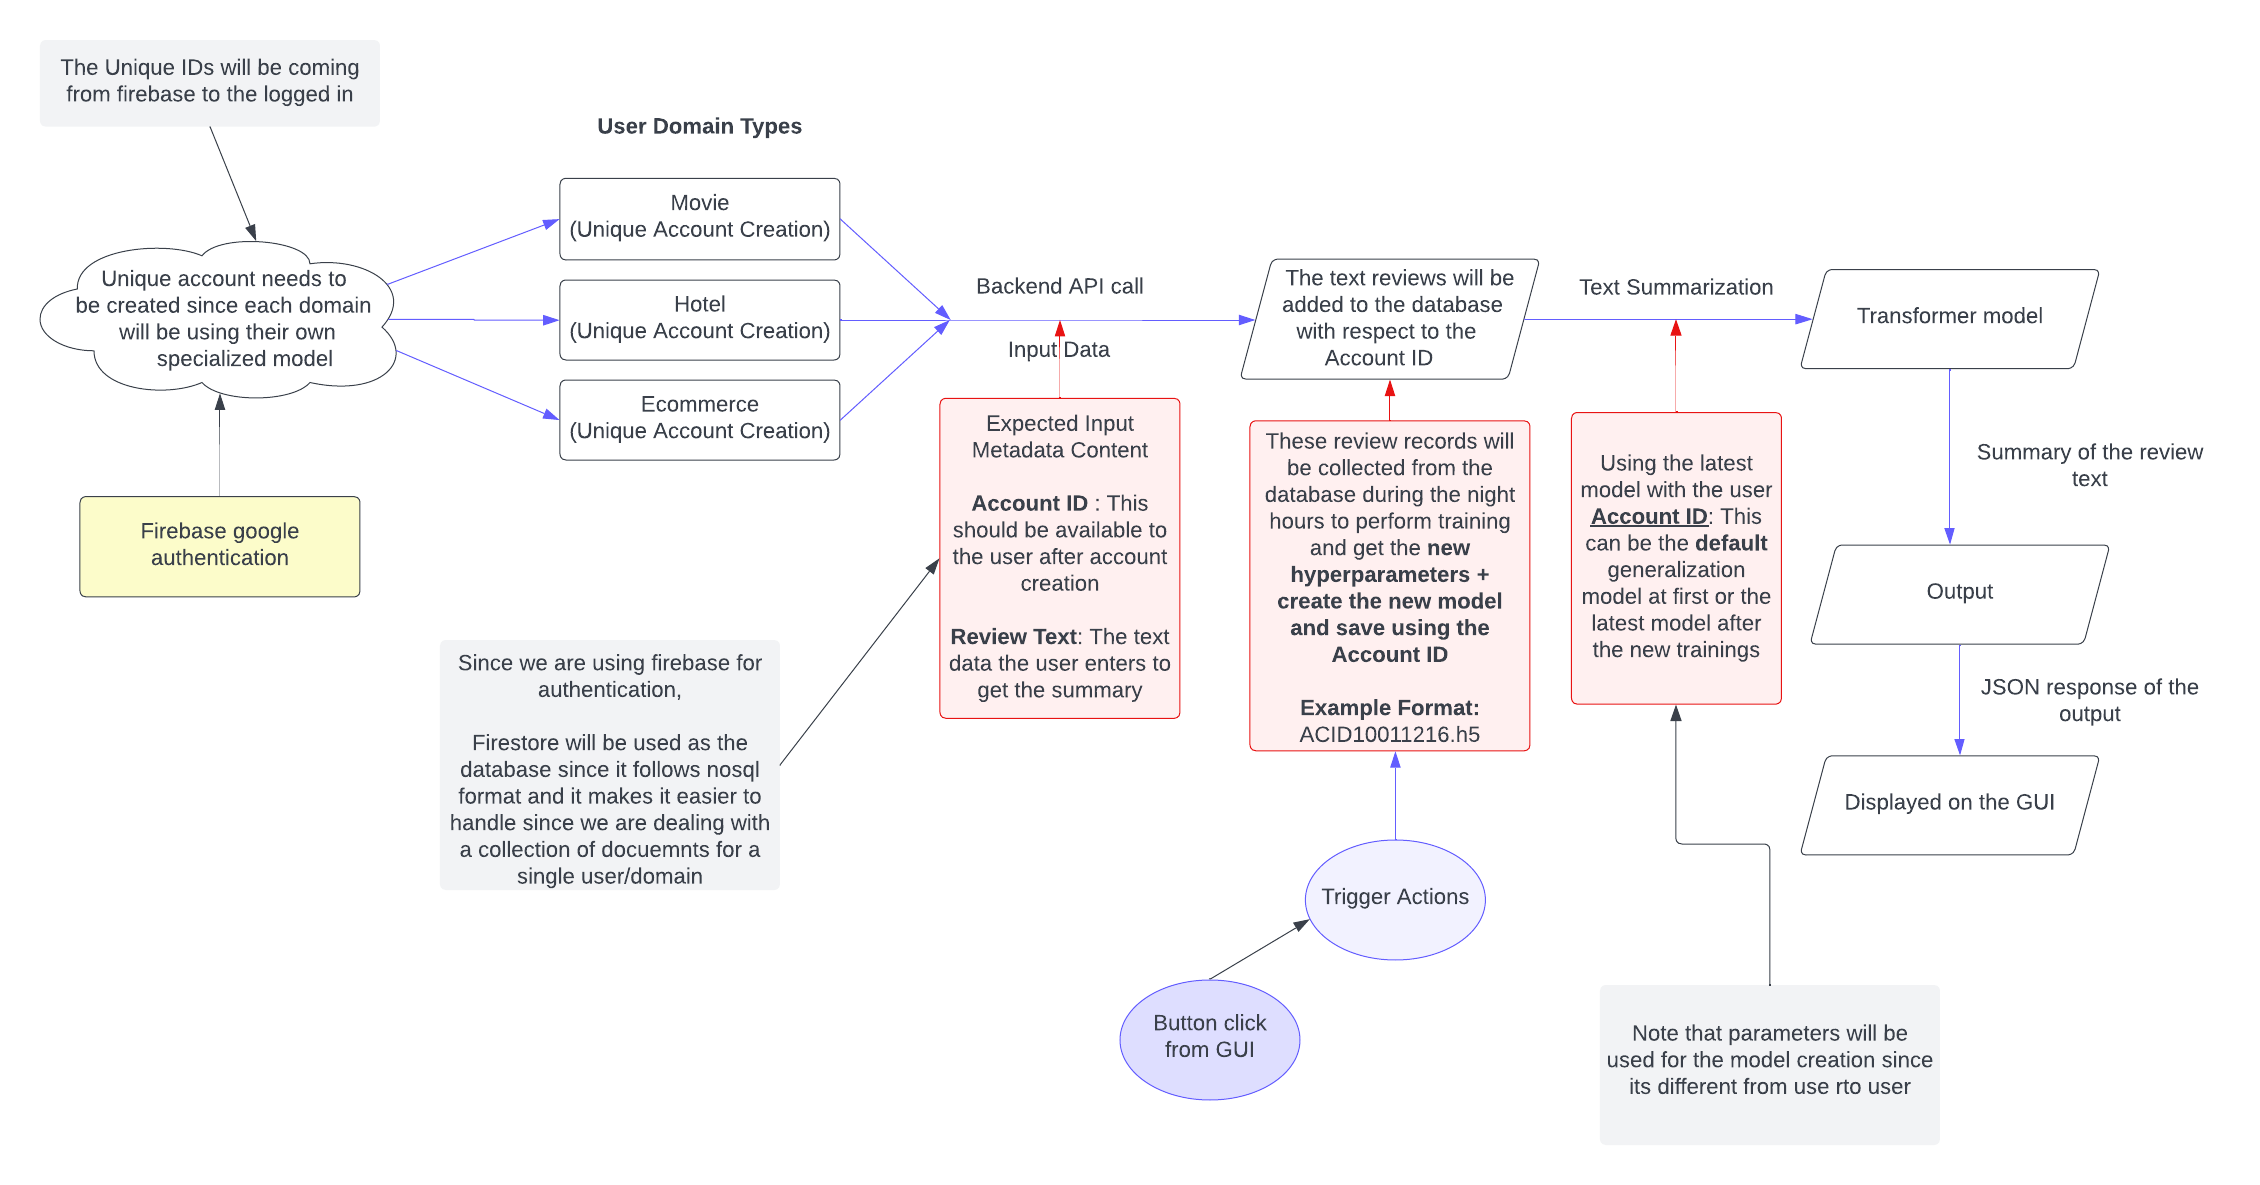
\includegraphics[width=\linewidth]{images/LR-Proposed Archtecture.png}}
\caption{Proposed Generalized Abstractive Summarization System Architecture}
\label{fig:trait-content-output}
\end{figure}

\section{Evaluation}
A machine learning model's performance, as well as its advantages and disadvantages, are understood through the process of model evaluation, which employs many evaluation measures. During the early stages of research, it's critical to evaluate models to determine their efficiency.

ROUGE also known as Recall-Oriented Understudy for Gisting Evaluation. Measures are made by comparison between an automatically generated summary/translation against a group of reference summaries (generally human-created summaries) \cite{lin_2004}.  ROUGE measures the recall, (according to how frequently the terms from the summaries created by humans appeared in those computers - generated.)


\begin{figure}[htbp]
\centerline{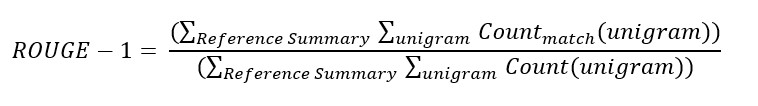
\includegraphics[width=\linewidth]{images/rouge-1.jpg}}
\caption{Rouge-1 Score Equation}
\label{fig:trait-content-output}
\end{figure}

\begin{figure}[htbp]
\centerline{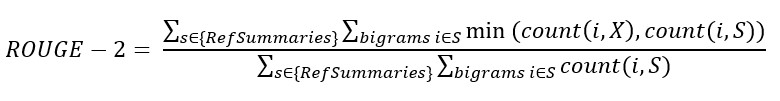
\includegraphics[width=\linewidth]{images/rouge-2.jpg}}
\caption{Rouge-2 Score Equation}
\label{fig:trait-content-output}
\end{figure}

\begin{figure}[htbp]
\centerline{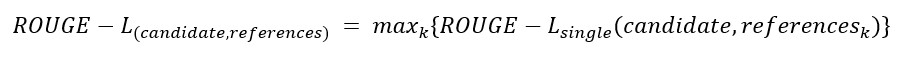
\includegraphics[width=\linewidth]{images/rouge-l.jpg}}
\caption{Rouge-L Score Equation}
\label{fig:trait-content-output}
\end{figure}

BLEU also known as Bilingual Evaluation Understudy is a metric used for the evaluation of the quality of machine-generated text by comparing it with a reference text that is supposed to be generated. \cite{steinberger_ježek}. BLEU measures the precision (as to how many words in the generated summaries appeared in the human-generated summaries)

\begin{figure}[htbp]
\centerline{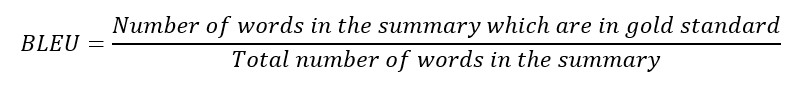
\includegraphics[width=\linewidth]{images/bleu-score.jpg}}
\caption{BLEU Score Equation}
\label{fig:trait-content-output}
\end{figure}

The ROUGE score was used as the final evaluation metric for this research since the weightage of it is the best metric for this research as proven by previous work.

BART, T5 \& Pegasus transformer architecture was experimented with for this research, out of which Bart gave the optimal results whereas T5 came close however Pegasus failed, there can be several reasons why Pegasus failed one of which can be due to the difference in the model architecture and the type of problem it can solve with respect to the dataset. 

\begin{figure}[htbp]
\centerline{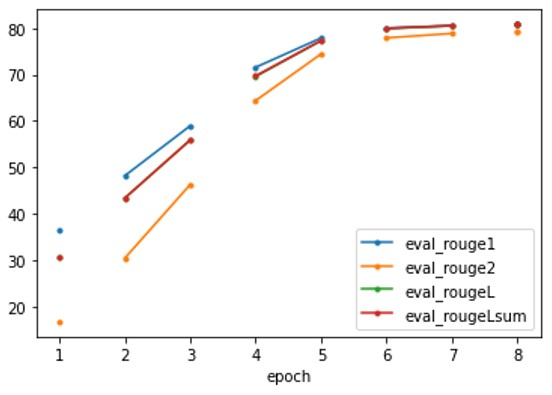
\includegraphics[width=\linewidth]{images/bart-model-validation-accuracy.jpg}}
\caption{Validation accuracy by the number of epochs - BART Model}
\label{fig:trait-content-output}
\end{figure}

\begin{figure}[htbp]
\centerline{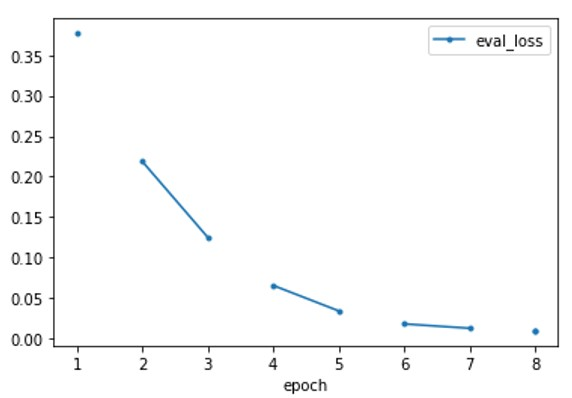
\includegraphics[width=\linewidth]{images/bart-model-validation-loss.jpg}}
\caption{Validation loss by the number of epochs - BART Model}
\label{fig:trait-content-output}
\end{figure}

ROUGE1 of 80.8, ROUGE2 of 79.42, ROUGE L of 80.8, and ROUGELSUM of 80.8 was the optimal evaluation metric result achieved from the BART model giving the best result.

\section{Future Enhancements}
Future Enhancements for text summarization models can be achieved through the use of transformer hybridization. This approach could lead to improved performance, enabling the models to better handle complex natural language processing tasks. Another potential improvement is the inclusion of text paraphrase models for user reviews. 

This would help to address the potential issue of inaccuracies in user-generated content. Additionally, applying keyword extraction for sentiment classification in review summaries could provide valuable insights for domain users to improve their services. 

By identifying which keywords contributed to the sentiment classification, businesses can understand their customers better and make informed decisions to enhance their services. These advancements can significantly benefit the field of natural language processing and improve the accuracy and efficiency of text summarization models.

\section{Conclusion}
% mention something about human-computer interaction here to make this related to the conference (add to the end of intro/ abstract too?)
The conclusion of this study finds that the author was able to design, build, and evaluate an adaptive generalized abstractive text summarization system using optimized transformers and automated hyperparameter tuning and model retraining with respect to any domain.


\printbibliography %Prints bibliography

\end{document}
